\documentclass[11pt,a4paper]{article}
\usepackage[T1]{fontenc}
\usepackage[utf8]{inputenc}
\usepackage{lmodern,microtype}
\usepackage[margin=25mm,headheight=15pt]{geometry}
\usepackage{amsmath,amssymb,booktabs,tabularx,array,longtable}
\usepackage[table]{xcolor}
\usepackage[numbers,sort&compress]{natbib}
\usepackage{enumitem}
\usepackage{placeins}
\usepackage{graphicx}
\usepackage{fancyhdr}
\usepackage{xurl}
\usepackage{hyperref}
\usepackage{bookmark}
\definecolor{ink}{HTML}{17324D}
\definecolor{accent}{HTML}{087E8B}
\definecolor{pale}{HTML}{EFF5F7}
\hypersetup{colorlinks=true,linkcolor=ink,citecolor=accent,urlcolor=accent,
  pdftitle={Artificial Life: Substrates, Evolutionary Dynamics, and Open-Endedness},
  pdfauthor={TIDE Research Notes}}
\urlstyle{same}
\setlength{\parindent}{0pt}
\setlength{\parskip}{5pt plus 1pt}
\setlength{\emergencystretch}{2em}
\renewcommand{\topfraction}{0.9}
\renewcommand{\textfraction}{0.08}
\renewcommand{\floatpagefraction}{0.8}
\setcounter{topnumber}{3}
\makeatletter
\setlength{\@fptop}{0pt}
\setlength{\@fpsep}{18pt}
\makeatother
\widowpenalty=10000
\clubpenalty=10000
\setlist{nosep,leftmargin=*}
\renewcommand{\arraystretch}{1.18}
\pagestyle{fancy}
\fancyhf{}
\fancyhead[L]{\small\textcolor{ink}{ARTIFICIAL LIFE}}
\fancyhead[R]{\small TIDE research review}
\fancyfoot[C]{\thepage}
\renewcommand{\headrulewidth}{0.3pt}
\newcolumntype{Y}{>{\raggedright\arraybackslash}X}
\newcommand{\model}[1]{\textsc{#1}}

\begin{document}
\hypersetup{pageanchor=false}
\begin{titlepage}
\vspace*{15mm}
{\small\sffamily\textcolor{accent}{RESEARCH REVIEW \quad | \quad NOVEMBER 2026}\par}
\vspace{10mm}
{\Huge\bfseries\textcolor{ink}{Artificial Life}\par}
\vspace{4mm}
{\LARGE Substrates, Evolutionary Dynamics,\\and the Problem of Open-Endedness\par}
\vspace{10mm}
{\large A narrative review of soft, hard, and wet artificial life\par}
\vspace{12mm}
\textbf{Abstract}\par
Artificial life studies how life-like organization can be constructed, maintained,
and transformed in computational, robotic, and biochemical systems. Its methods
span executable replicators, cellular automata, evolving robots, collective
machines, protocells, and minimal cells. This review compares these approaches
through their units of heredity, sources of variation, reproductive constraints,
physical embodiment, and experimental observables. It distinguishes
self-organization from self-reproduction, externally optimized discovery from
endogenous evolution, and finite adaptive change from claims of open-endedness.
Particular attention is given to ecological feedback, spatial organization,
constructed boundaries, conserved flows, operational individuality,
measurement, and reproducibility. Recent work on computational replicator
detection and foundation-model-assisted search sharpens these distinctions
without removing the need for causal tests. A final section translates the
comparison into research questions for TIDE, a planned digital-life kernel.
The review reports literature evidence and design proposals. Original diagrams
clarify mechanisms; a separate appendix reanalyzes archived exploratory
prototype outputs. No new simulation, robotics, or laboratory runs were made
for this review.
\vfill
\textbf{Scope and status}\par
English narrative review; literature search dated 15 November 2026.
Representative primary studies and selected field syntheses are included.
Coverage is broad but not systematic or exhaustive. Preprints, limited-access
sources, and project-specific proposals are identified explicitly.\par
\vspace{6mm}
{\small Prepared in the TIDE research workspace. Bibliographic provenance and
local reference-cache metadata accompany the source.\par}
\end{titlepage}
\pagenumbering{roman}
\hypersetup{pageanchor=true}
{\small\setlength{\parskip}{0pt}\tableofcontents}
\clearpage
\pagenumbering{arabic}
\section{Scope, method, and conceptual framework}
\subsection{A constructive study of life-like processes}
Artificial life asks what kinds of organization can arise when components are
given explicit rules of interaction, reproduction, development, or maintenance.
The field's computational (soft), robotic (hard), and biochemical (wet) approaches
are overlapping experimental methods, rather than successive levels of
achievement \citep{Aguilar2014}. A robot can be evolved in simulation and then
manufactured; a biochemical population can be controlled by software. The
substrate therefore does not, by itself, identify what a study demonstrates.

This review emphasizes soft artificial life, the setting of the TIDE project,
while retaining substantive comparisons with physical machines and chemical
systems. Its organizing questions are: what persists, what is reproduced, what
can vary, which consequences affect reproduction, and who or what supplies the
conditions for continuation? These questions make apparently similar claims
comparable without requiring a single all-or-nothing definition of life.

\subsection{Search strategy and evidence limits}
The search was conducted on 15 November 2026. It began with cached studies of
Tierra, Avida, evoloops, Stringmol, computational replicators, and open-ended
evolution, then followed three parallel streams: recent frontiers, stagnation
and measurement, and spatial/update semantics. Additional searches covered
cellular-automata foundations, embodied systems, and chemical construction.
Original papers, author and institutional copies, and official repositories
were preferred. Field reviews provide taxonomy; experimental claims are tied
to the relevant primary work. Exact queries and reading-depth notes accompany
the LaTeX source in the repository's research records.

This is a narrative review, not a systematic review or meta-analysis. Selection
favored studies that expose mechanisms, causal controls, or informative failure
cases. It does not establish that omitted systems lack relevant capabilities.
Versioned preprints are distinguished from journal articles. Where only
indexed primary-text passages or publisher previews were accessible, that
limitation is stated. No reported experiment was independently reproduced.
Comparisons across substrates are analytical interpretations, not quantitative
rankings on a common benchmark.

\subsection{Separate capabilities before comparing systems}
Self-organization denotes the formation of macroscopic structure through local
interactions. Self-maintenance concerns persistence under disturbance and
turnover. Self-reproduction additionally requires a causal process producing
another instance of the relevant organization. Evolution is heritable population
change, which can involve selection or drift. Natural selection specifically
concerns trait-dependent differences in reproductive success. None of these terms
automatically establishes continuing innovation \citep{Taylor2016}.

The distinctions are operational. A moving pattern can persist without
reproducing. A designed loop can reproduce without generating an evolving
population. A trained local rule can repair a shape while its parameters remain
fixed. A genetically simplified cell can divide while depending on a rich
external environment. These are informative achievements, but different ones.

Three layers should also remain distinct: the transition rules of a substrate,
the processes occurring within it, and the observer or search procedure used to
find and evaluate those processes. This distinction becomes especially useful
when comparing digital ecology with modern optimization-assisted discovery.
An external objective can be scientifically valuable without being mistaken
for a reproductive advantage generated inside the studied world.

\begin{table}[htbp]
\centering\small
\caption{Substrate classes and the questions their evidence can address. The
last column identifies a limit of inference, not a judgment of research value.}
\begin{tabularx}{\textwidth}{@{}>{\raggedright\arraybackslash}p{17mm}YYY@{}}
\toprule
Approach & Experimental object & Characteristic strength & Inference requiring more evidence \\
\midrule
Soft & Programs, automata, simulated agents and reactions & Explicit interventions, complete state access, controlled replay & Biological feasibility; physical autonomy; indefinite innovation \\
Hard & Embodied robots, manufactured structures and collectives & Contact with material dynamics, sensing, actuation and fabrication & Autonomous reproduction or evolution beyond an external optimizer \\
Wet & Compartments, catalysts, genomes and cells & Actual chemical compatibility, material turnover and biochemical heredity & A complete autonomous life cycle from separately demonstrated modules \\
\bottomrule
\end{tabularx}
\label{tab:substrates}
\end{table}


\section{Soft artificial life: substrates and evolutionary mechanisms}
Figure~\ref{fig:substrates} distinguishes the local transition units before
comparing their reproductive or evolutionary capabilities.
\begin{figure}[!htbp]
\centering
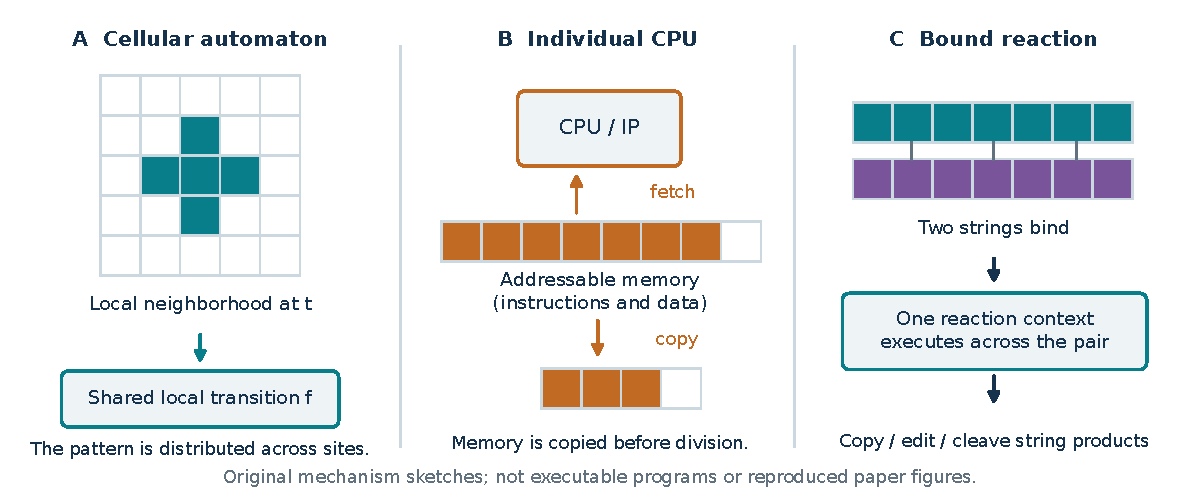
\includegraphics[width=\textwidth]{figures/soft-substrates.pdf}
\caption{Three computational substrates, drawn as original mechanism sketches
from the descriptions of cellular automata, Tierra, and spatial Stringmol
\citep{Langton1984,Ray1991,Hickinbotham2021}. The highlighted CA neighborhood is
not a reproducing loop. Tierra separates CPU ownership from code location;
Stringmol executes through a bound-pair reaction context. The panels do not
assert equivalent reproduction or evolutionary capabilities.}
\label{fig:substrates}
\end{figure}
\subsection{Discrete cellular automata and construction}
A cellular automaton specifies a spatial state and a local transition, commonly
written schematically as
\begin{equation}
 x_i(t+1)=f\!\left(x_j(t):j\in\mathcal N(i)\right).
\end{equation}
The neighborhood, boundary conditions, state alphabet, and update schedule are
parts of the model. Simple local descriptions can support elaborate structures,
but visual elaboration alone does not identify reproduction or heredity.

Langton's engineered self-reproducing loop demonstrates that a compact local
construction process need not be a universal constructor
\citep{Langton1984}. Its circulating information participates in constructing
and copying a new loop. The result concerns an explicit reproduction mechanism;
it does not establish spontaneous origins or indefinitely diversifying
descendants. Evoloops add an instructive contrast: interaction and collision
under deterministic rules can alter reproducing structures and generate
inherited variation \citep{Sayama1998,SayamaNehaniv2024}. Reported size
convergence also shows why an evolving population is not sufficient evidence
of ongoing novelty.

These systems make a central point for kernel design. Variation need not always
be an externally sampled mutation event: it can result from ordinary
interactions in the substrate. Conversely, declaring a rule local does not
make its consequences unstructured by design. The state alphabet and
transition table already determine which constructions are possible.

\subsection{Executable digital organisms: Tierra and Avida}
Executable-genome systems place variation inside programs whose operations
affect their own continuation. Tierra uses a shared memory environment and
individual execution contexts; allocation, copying, and division participate
in reproduction \citep{Ray1991}. Execution ownership and code location are
distinct: an individual's CPU can execute another individual's instructions.
This separation permits dependencies and redirection of copying that a
high-level ``duplicate self'' operation would conceal. Memory permissions,
scheduling, and reclamation still define the interaction opportunities.

Avida supplies a complementary experimental platform with individual virtual
hardware and configurable environments \citep{OfriaWilke2004}. Task rewards,
mutation, and spatial settings can be controlled explicitly. This supports
causal experiments, while also making it necessary to state which advantages
were supplied by the investigator. A complex task evolving under a task-based
environment is not the same claim as an unprescribed replication strategy
arising through competition for space and execution time.

For comparison, a digital organism should not be identified only with its byte
string. Its reproductive consequences depend on interpretation, CPU state,
accessible memory, neighbors, and scheduling. Nor should a single graph called
``ancestry'' silently combine all causal channels. The individual initiating a
division, the provider of executed instructions, and the donor of copied bytes
can differ. Separating these channels makes borrowing and redirection
experimentally testable without assigning ecological roles in advance.

\begin{figure}[!htbp]
\centering
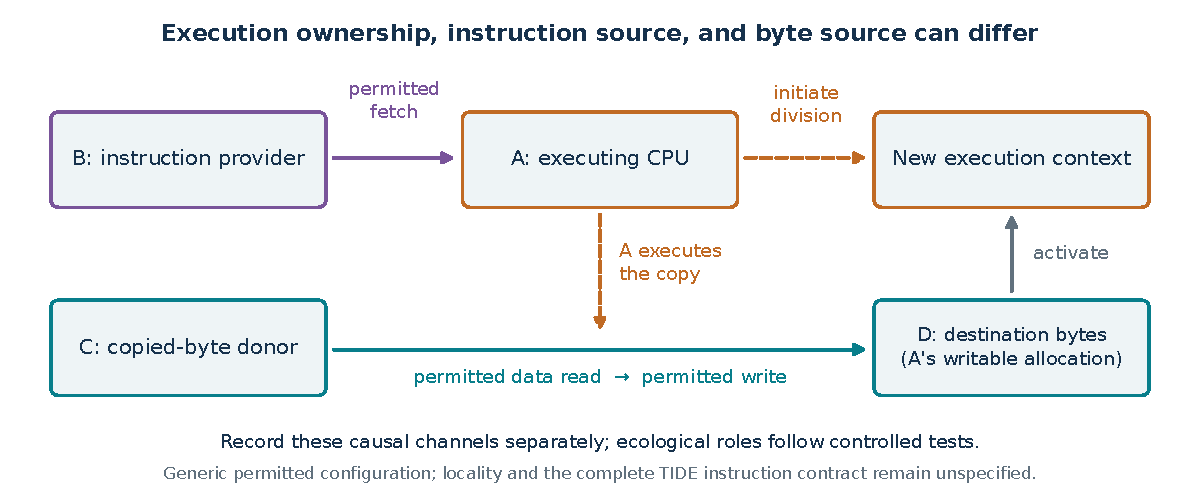
\includegraphics[width=\textwidth]{figures/replication-provenance.pdf}
\caption{Separate causal channels in a generic permitted VM configuration.
A executes instructions supplied by B, copies bytes supplied by C into its
writable allocation D, and initiates division. The diagram extends the
distinctions motivated by Tierra's borrowed copying routines and redirected
copying \citep{Ray1991}; it is neither a recorded three-party Tierra event nor
an approved TIDE contract. Solid colored arrows show instruction/data flow;
dashed arrows show actions of A's execution context.}
\label{fig:provenance}
\end{figure}
Figure~\ref{fig:provenance} explains why byte agreement alone cannot identify
the reproductive mechanism or a unique causal parent.

\subsection{Artificial chemistries and evolving replication reactions}
Artificial chemistries formulate interactions in terms of components and
reaction processes. The important choice is whether a reaction is prescribed
as a fixed transformation or constructed through executable interactions.
Spatial Stringmol is especially relevant to the latter: neighboring strings
bind, execute a reaction, and produce or modify strings
\citep{Hickinbotham2021}. A bound pair is an execution unit, unlike Tierra's
separate CPU ownership. Control flow and copying operations can change how
replication proceeds, rather than changing only a scalar replication rate.

The observed evolution of recognition and copying strategies motivates tests
of functional relationships. It does not imply that a particular ecological
role must survive. Extinction and the later loss of expensive strategies are
part of the evidence. A label such as parasitism should describe consequences
in a stated interaction context, rather than cause those consequences through
special protection, resource transfers, or replacement rules in the kernel.

This distinction suggests a useful experimental progression. First establish
that small fixed programs can perform ordinary self-copy, use another
program's instructions, and redirect copying to a different permitted source.
Then test whether variation produces such pathways and whether their
reproductive effects persist. Expressibility, appearance, and ecological
establishment answer different questions.

\subsection{Origins of replicators and their subsequent spread}
The computational-life experiments of Ag\"uera y Arcas and colleagues examine
replication arising among interacting programs, including conditions without
background mutation \citep{Aguera2024}. Their examples broaden the range of
computational substrates in which replication can arise. They do not remove
the distinction between a first replicator, successful expansion, and the
later evolution of new strategies.

A 2026 BFF follow-up makes that distinction more directly measurable
\citep{Knierim2026}. Under its tested program distributions and detector,
simple random processes can compete with interaction-based searches for
replicators. The detector itself has finite-chain and alignment limitations.
Consequently, origins should be evaluated with explicit candidate replay and
appropriate null searches, while takeover requires a separate population
measurement. These results concern particular short-tape substrates, not a
general theorem about the value of interaction or recombination.

For a supplied-ancestor experiment, the starting question is different:
replication already exists, and the investigator asks what heritable
strategies and dependencies appear afterward. Mixing the two objectives makes
failure difficult to interpret. Failure to find an ancestor in random bytes
need not invalidate a study of evolution after an ancestor; successful spread
of that ancestor does not establish an account of origins.

\subsection{Continuous and neural cellular substrates}
Lenia extends cellular-automata exploration through continuous-valued states,
weighted neighborhoods, and incremental growth rules \citep{Chan2019}. The
2019 study catalogues persistent and moving organizations, while explicitly
leaving self-replication undiscovered in that work. Human-guided exploration
of parameters and initial conditions is therefore distinct from reproduction
and selection within an autonomous population. Later variants must be judged
on their own evidence rather than inheriting either a capability or a
limitation from the original system.

Flow-Lenia introduces mass-conserving dynamics and localized rule parameters
that can interact within one world \citep{Plantec2025}. Directed optimization
and intrinsic evolutionary experiments remain separate parts of the work.
Its measures also expose an interpretive problem: raw activity and
mass-normalized activity can order treatments differently. A parameter vector
used as a species identifier is an operational choice, not an independently
established unit of individuality.

Neural cellular automata address another capability: learning a shared local
rule that develops and repairs a target configuration
\citep{Mordvintsev2020}. The training loss and training distribution are supplied
externally. Distributed deployment and damage recovery demonstrate local
developmental control, not necessarily inherited rule variation or
reproduction-driven evolution during deployment. This separation helps avoid
using ``growth,'' ``regeneration,'' and ``evolution'' interchangeably.

\subsection{External search and AI-assisted discovery}
ASAL uses foundation-model representations to guide searches over artificial-life
simulations \citep{Kumar2025}. Such a search can discover configurations aligned
with a prompt or a chosen novelty/diversity criterion. The representation,
renderer, search algorithm, and evaluation horizon jointly determine which
discoveries are favored. This makes the approach a tool for exploring
substrates, while its evaluator remains outside their internal ecology.

The extended Flow-Lenia exploration study similarly distinguishes
curiosity-driven configuration search from dynamics within a selected
configuration \citep{Michel2026}. Larger or more active simulations require
normalization and longer observation before their apparent complexity can be
interpreted. Search coverage, visually novel trajectories, and endogenous
adaptive innovation should therefore be reported as separate outcomes.

\begin{table}[htbp]
\centering\small
\caption{Selected soft systems compared by their experimental unit and the
claim requiring further evidence. Entries describe the cited studies, not
every implementation or later variant.}
\begin{tabularx}{\textwidth}{@{}>{\raggedright\arraybackslash}p{25mm}YY@{}}
\toprule
System & Main unit or mechanism & What does not follow automatically \\
\midrule
Langton loop & Constructed reproducing pattern & Heritable diversification \\
Evoloop & Interacting reproducing structures & Continuing novelty after convergence \\
Tierra & Executable genome and individual CPU & Unbounded strategy or complexity growth \\
Avida & Configurable digital organisms & Task-independent ecological innovation \\
Stringmol & Executable bound-pair reaction & Universal coexistence or complexity growth \\
BFF & Interacting program tapes & Origin, takeover and innovation being one event \\
Lenia / Flow-Lenia & Continuous local dynamics and, in Flow-Lenia, localized parameters & Morphological diversity identifying evolutionary individuals \\
Neural CA / ASAL & Trained rules or externally searched configurations & Autonomous Darwinian evolution during deployment \\
\bottomrule
\end{tabularx}
\label{tab:soft}
\end{table}

\FloatBarrier
\section{Hard artificial life: embodiment, adaptation, and collective construction}
\label{sec:hard-life}

Hard artificial life places synthetic organization in physical machines, where
structure, control, contact, and available power jointly determine behavior.
Its relevance to a predominantly soft-ALife review is methodological: embodiment
tests which modeled mechanisms survive material implementation. Three primary
studies illustrate distinct achievements---evolutionary design, adaptation within
an individual's lifetime, and distributed construction. They do not collectively
establish an autonomous population of reproducing robots. Keeping these
achievements separate makes their contributions easier to compare with digital
evolution.

\subsection{Joint evolution of morphology and control}

\citet{hardlipson2000} evolved robotic bodies and neural controllers together in
simulation. Mutation added, removed, or modified structural and control
components; selection rewarded displacement over a prescribed interval. Selected
designs were converted into printable structures and fabricated in thermoplastic,
after which motors were inserted manually. Three physical examples produced
locomotion corresponding to their simulated mechanisms. This demonstrated a
connection between evolutionary search and physical fabrication, with morphology
and control selected as integrated units rather than treating the body as fixed.

Transfer was imperfect. The manuscript's Table~I reports substantial distance
differences for two examples, attributed to slipping and an inadequate friction
model. The \emph{reality gap} is therefore visible within this demonstration:
qualitative transfer of a mechanism need not preserve quantitative performance.
Its autonomy also has a defined boundary. Fitness evaluation and selection took
place in simulation; fabrication used supplied equipment and materials, and
assembly retained a human step. The study supports automated embodied design,
not an ecological population manufacturing its own descendants
\citep{hardlipson2000}.

\subsection{Self-modeling and adaptation after damage}

\citet{hardbongard2006} investigated a different problem: recovering useful
behavior after an existing robot's body changes. A four-legged robot alternated
physical actions with synthesis of candidate body models. Exploratory actions
were chosen to distinguish competing models; a selected model then supported
optimization of a locomotion sequence. After part of a leg was removed, revised
models enabled an alternative gait. Comparisons against two random-exploration
baselines used the same number of physical actions, and model-driven exploration
improved inference within the tested hypothesis space.

The distinction from Darwinian evolution is central. Competing internal models
and optimized actions belong to an adaptation procedure, not a lineage of
reproducing physical individuals. Furthermore, the model family was constrained:
after damage, topology remained fixed while limb dimensions could change. The
reported locomotion demonstration used a model selected from repeated modeling
experiments. These qualifications retain the achievement---active inference can
guide compensatory behavior---while avoiding a claim of unrestricted self-knowledge,
physical regeneration, or inherited evolutionary improvement
\citep{hardbongard2006}.

\subsection{Distributed rules and externally specified collective form}

\citet{hardrubenstein2014} demonstrated programmable shape formation with
1024 Kilobots. Local communication, distance estimation, edge following,
gradients, and distributed localization supported assembly despite noisy motion
and sensing. Each robot received the same algorithm and target-shape image;
a user positioned four specially programmed seed robots to establish the
assembly's origin and orientation. The full swarm formed two shapes, each in
roughly twelve hours. Additional smaller-swarm trials examined consistency and
accuracy. Reported trials completed without charging, reprogramming, or other
human intervention during execution, although final shapes showed warping and
packing defects.

This is a strong demonstration of decentralized execution under physical
variability. It is also compatible with centralized specification of the desired
outcome: local interactions implement a supplied objective. The resulting
arrangement reorganizes existing robots; it does not manufacture new robots or
transmit variable inherited programs through reproduction. The paper also treats
physical attachment into stable structures as a future direction. Consequently,
``self-assembly'' here should be read according to the demonstrated collective
shape-formation task, rather than as evidence for a self-producing machine
organism \citep{hardrubenstein2014}.

\subsection{What embodiment contributes to soft artificial life}

The following comparison is a synthesis of these cases, not an additional
experimental result. A useful transfer is to examine the coupling between an
individual's organization and the operations available to it. In soft systems,
representation, instruction semantics, and environmental access jointly delimit
what can evolve, just as body and controller jointly delimit robotic behavior.
Interventions can ask which apparent capability disappears when one coupling is
changed. Adaptive performance should also be separated from its mechanism:
within-lifetime learning, population selection, and a designer's search may all
improve an observable score through different causal processes.

Physical embodiment additionally requires an explicit accounting boundary.
Feedstock, manufacturing equipment, electronics, power supplies, and maintenance
cannot be omitted when evaluating material autonomy. A robot's operational
independence during a trial does not close its production cycle. Soft experiments
can similarly state which resources and services their environment supplies, but
a digital resource budget is not thereby a measurement of physical energy or
manufacturing feasibility. Conversely, hardware noise need not be copied into a
digital kernel merely to make it appear biological. The transferable requirement
is to justify the abstraction and test sensitivity to it.

These historical exemplars therefore contribute tests of realization,
adaptation, and collective reliability to the review's main computational focus.
They provide neither a universal recipe for artificial life nor evidence that
open-ended evolution follows from embodiment. This bounded selection does not
survey the full contemporary frontier of evolutionary robotics.

\section{Wet artificial life: construction, replication, and integration}
\label{sec:wet-life}

Wet artificial life investigates life-like organization in biochemical systems.
Bottom-up work constructs selected functions from molecular components;
top-down work simplifies or redesigns existing cells. Their achievements concern
distinct functions: compartment growth, molecular replication, cellular
reproduction, or adaptation. Membrane division does not demonstrate genome
copying; genome synthesis does not establish construction of every cellular
component from nonliving materials
\citep{wetZhu2009,wetGibson2010,wetHutchison2016}.

\subsection{Compartments: reproduction without a complete genetic system}

Zhu and Szostak demonstrated coupled growth and division of model protocell
membranes. Fatty-acid vesicles supplied with membrane material developed
elongated shapes that divided under modest fluid shear. Repeated cycles were
possible, and encapsulated RNA was redistributed into daughter compartments
without the substantial leakage associated with their comparison method
\citep{wetZhu2009}. The result establishes a physical route linking boundary
growth, division, and retention of contents, rather than treating division as an
unrelated operation imposed after growth.

The distinction between distributing RNA and replicating it is essential.
The study did not demonstrate an internally replicating genome coupled to the
membrane cycle. Its Discussion explicitly identifies that integration as a
further requirement for a more complete protocell. Membrane precursors and
mechanical agitation remained externally supplied. The experiment isolates a
tractable physical problem; its success does not establish cellular autonomy
or sustained adaptive evolution \citep{wetZhu2009}.

\subsection{Chemical replication and limited evolutionary dynamics}

Lincoln and Joyce constructed RNA enzymes that catalysed one another's
production from supplied component substrates. The cross-catalytic system
supported exponential amplification without proteins in the replication
reaction. When related replicators competed for shared substrates, recombinant
variants arose and became abundant \citep{wetLincoln2009}. This provides a
chemical example in which replication machinery participates in the system
being reproduced, and in which heritable differences affect competitive
outcomes. It goes beyond observing a persistent structure or merely counting
more molecules.

Here, ``self-sustained'' describes a catalytic cycle conditional on substrate
replenishment, rather than synthesis of those substrates, membrane maintenance,
or environmental control. The enzymes had also undergone prior experimental
optimization. The authors characterize their genetic system as restricted and
identify the emergence of new encoded functions beyond replication as an open
challenge. Thus the work demonstrates a bounded form of chemical evolution,
not open-ended functional innovation or a complete account of life's origin
\citep{wetLincoln2009}. It offers a useful comparison for digital replicators:
the source of building blocks and the allowed variation determine which
evolutionary claims the observed competition can support.

\subsection{Synthetic genomes and top-down minimal cells}

Gibson and colleagues demonstrated cells controlled by a chemically synthesized
bacterial chromosome after its introduction into a recipient cell. Descendants
reproduced with the synthetic genome and exhibited the expected phenotypic
properties \citep{wetGibson2010}. The achievement concerns genome construction
and control of an existing cellular system. The paper explicitly states that
the recipient cytoplasm was not synthetic. Inherited cellular machinery matters
to initial establishment, although its original molecules are progressively
replaced in descendants.
Genome-directed renewal and construction of an entire cell from nonliving
components remain distinct experimental claims.

Hutchison and colleagues subsequently minimized a synthetic bacterial genome
through iterative design and testing. Their initial design was not viable;
retaining genes needed for robust growth helped produce a viable reduced
genome, which still included genes of unknown biological function
\citep{wetHutchison2016}.\footnote{The account of this study is limited to
the authors' published abstract and institutional publication record;
the detailed full text was not inspected in this review pass.}
This is an empirical approach to minimality: successful reproduction tests
whether a reduced system remains viable under its experimental conditions.
The unresolved gene functions also distinguish a small working cell from a
fully understood cell. Genome size alone supplies neither a complete causal
explanation nor a universal lower bound for every environment or lineage.

\subsection{Minimality does not remove the capacity to adapt}

A later experiment directly examined evolution in a genomically minimized
cell. Moger-Reischer and colleagues compared minimal and non-minimal strains
using mutation measurements, laboratory evolution, fitness assays, and genome
analysis. The minimized strain recovered fitness lost through streamlining,
while some phenotypic responses depended on genomic context
\citep{wetMogerReischer2023}. This demonstrates that severe reduction need not
eliminate adaptive potential. It also changes the question from whether a
designed genome functions initially to how its descendants respond to selection.

The cells inherited biological organization and received externally maintained
culture conditions and supplies. Adaptation over the observation period does
not establish spontaneous origin, environmental independence, or indefinitely
expanding complexity \citep{wetMogerReischer2023}.

\subsection{The integration problem and its relevance to digital models}

Together, these studies identify a methodological tradeoff. Isolated bottom-up
systems make particular mechanisms easier to attribute, while retaining fewer
integrated cellular functions. Top-down cells reproduce and adapt as complete
organisms, but inherit machinery and organizational history that the experiment
does not reconstruct. The comparison is therefore about which dependencies
have been explained, rather than which demonstration looks most life-like.
An integration claim must connect boundary maintenance, heritable replication,
resource acquisition, and reproduction within the same continuing system.

For soft artificial life, the transferable lesson is experimental accounting,
not a requirement to imitate cellular chemistry. A digital study should state
which processes its programs perform, which resources the environment supplies,
and which lifecycle transitions the simulator grants. Distinguishing a working
replication mechanism from establishment, adaptation, and continuing innovation
helps prevent a successful component demonstration from carrying a broader
claim than its evidence supports.

\section{Ecology, open-endedness, and experimental measurement}
\subsection{Space changes mechanisms, not only appearance}
Spatial organization can alter which interactions reproduce. Hypercycle and
replicator models demonstrate that waves and restricted mixing can protect
some productive organizations against exploitation
\citep{Boerlijst1991,Takeuchi2009}. Their catalytic relationships are prescribed,
so they do not establish that an instruction-level VM will generate the same
ecology. They do show why a well-mixed comparison and a spatial model can
select differently even when both sustain a population.

For executable systems, the corresponding hypothesis must be expressed in
operations: where a program can read, where copying reserves space, which
neighbors can exploit instructions, and how opportunities move across the
grid. A selected snapshot of a wave is insufficient. Measurements should
include invasion failure, extinction, spatial correlations, available space,
and the work spent on successful and unsuccessful reproduction.

\subsection{Scheduling and the meaning of reproducibility}
Update order is part of a dynamical model. The partially accessible study by
Sch\"onfisch and de Roos distinguishes several asynchronous procedures and
reports effects of update-order correlations \citep{Schonfisch1999}. Its
publisher preview supports the need to specify the algorithm; it is not used
here as a proof about a stochastic allocating VM. A fresh random permutation,
sampling sites with replacement, and event-driven waiting times are different
processes.

For a two-phase digital model, the transition can be described schematically as
\begin{align}
 I_t &= E(S_t;\theta,\xi_t),\\
 S_{t+1} &= R(S_t,I_t;\theta,\xi_t),
\end{align}
where $S_t$ is the full state, $I_t$ the proposed effects, $\theta$ the rule
configuration, and $\xi_t$ the designated random inputs. This is a conceptual
decomposition, not a complete TIDE specification. Read visibility, conflict
priority, reservation release, and newborn activation still require explicit
definitions.

Counter-based random generators can associate draws with logical events
instead of an order-dependent stream \citep{Salmon2011}. That supports replay
across execution partitions, but does not supply the event-identity mapping
or make ambiguous transitions deterministic. Reproducing identical state
hashes across implementations of one rule is a different claim from finding
similar ecological outcomes under different rules. Equal seeds do not make
synchronous and sequential models equivalent.

\begin{figure}[!htbp]
\centering
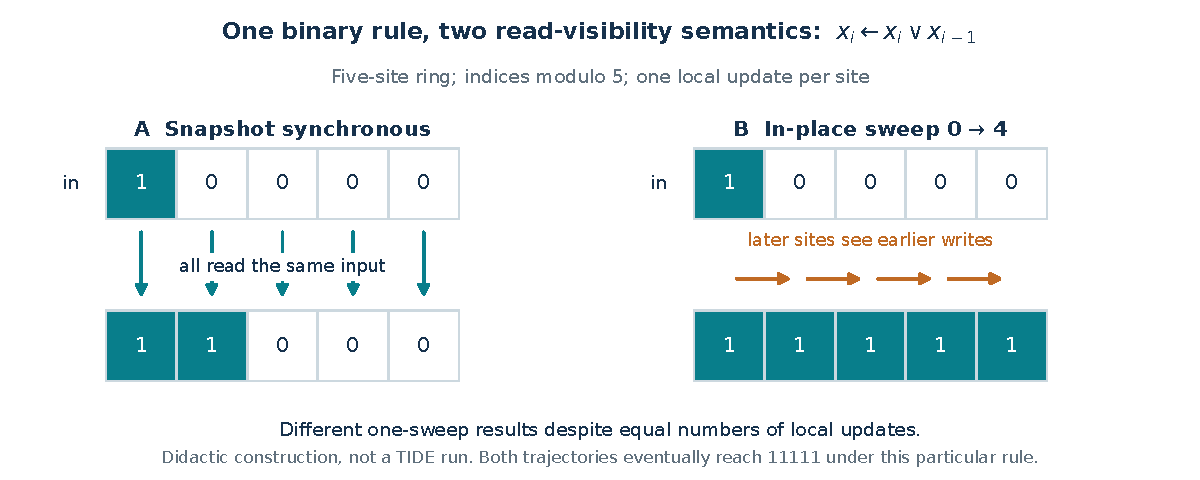
\includegraphics[width=\textwidth]{figures/update-semantics.pdf}
\caption{An original deterministic example of read visibility. With periodic
boundaries, $x_i\leftarrow x_i\lor x_{i-1}$ and initial state $10000$, one
snapshot-synchronous update yields $11000$; an in-place sweep in order
$0,1,2,3,4$ yields $11111$. Both perform five local evaluations. This constructed
example illustrates the scheduling distinction discussed above, not an
experiment from the cited literature or TIDE. Both eventually saturate under
this particular rule, so the immediate difference does not establish a
long-term ecological effect.}
\label{fig:scheduling}
\end{figure}
The finite example in Figure~\ref{fig:scheduling} isolates read visibility
without adding resource or mutation differences.

\subsection{Stagnation and functional change}
Program length, diversity, and complexity can move independently. Standish's
Tierra studies include size growth without growth in the measured complexity,
and a parsimony sweep whose limited improvements did not establish
open-endedness \citep{Standish2003,Standish2004}. A plateau therefore needs a
specified observable and observation horizon. Extinction is a separate outcome
from a surviving population whose reproductive behavior stops changing.

Responsive ecological feedback is one possible source of changing selective
conditions. Zaman and colleagues use frozen and replayed parasite controls to
distinguish responsive coevolution from exposure to a fixed collection of
opponents \citep{Zaman2014}. Their Avida setting defines infection and a suite
of logic tasks. The causal control is informative; the task-based complexity
measure and interaction rules do not transfer unchanged to task-free digital
ecology. Likewise, Chromaria's preliminary opportunity-creation ablation
motivates a hypothesis, not a universal necessity theorem
\citep{Soros2014}. Access to that paper in this review was limited to indexed
primary-text passages.

\subsection{Measure several properties instead of declaring a binary victory}
The open-ended-evolution workshop synthesis separates observable hallmarks
from proposed enabling mechanisms \citep{Taylor2016}. MODES develops
operational diagnostics for change, novelty, complexity, and ecology
\citep{Dolson2019}. Its filtering and component definitions are choices that
must remain visible. Persistence can help distinguish fleeting variation from
longer-lived contributions, but it does not exclude all drift. An informative
site count is context-dependent and can miss interactions among sites.

\begin{table}[htbp]
\centering\small
\caption{A measurement panel for soft artificial life. These are review
recommendations, not an approved event schema or a new fitness function.}
\begin{tabularx}{\textwidth}{@{}>{\raggedright\arraybackslash}p{28mm}YY@{}}
\toprule
Property & Observable example & Essential qualification \\
\midrule
Reproduction & Products and repeated viable descendants in replay & One copied fragment need not reproduce \\
Persistence & Descendants after declared lags; survival curves & Drift and spatial isolation can preserve lineages \\
Novelty & First observed behavioral signatures, separately from new byte strings & Recurrence and neutral variation can inflate turnover \\
Complexity & Contextual perturbation effects alongside program length & Length, indispensable sites and algorithmic complexity differ \\
Interaction & Focal reproduction alone, paired, and under controlled substitutions & Pair tests can miss higher-order or density-dependent effects \\
Spatial ecology & Invasion, wave persistence, spatial correlations and extinctions & A visually organized survivor can be an unrepresentative run \\
\bottomrule
\end{tabularx}
\label{tab:measurement}
\end{table}

At least three denominators should be considered when comparing treatments:
world steps, executed instructions, and occupied or available resources.
If two schedulers provide different work per step, equal step counts are not
equal computational exposure. If one treatment contains more organisms, more
new genotypes may simply reflect more reproductive events. Normalization
should answer a declared question, while retaining the raw observations.

Finite observation also creates censoring. A lineage born near the end of a
run has not had the same opportunity to pass a persistence threshold as an
early lineage. Its classification is unresolved, rather than automatically
unsuccessful. Genotype archives should include extinct variants, and sampling
limits should disclose which short-lived events can be missed.

\begin{figure}[!htbp]
\centering
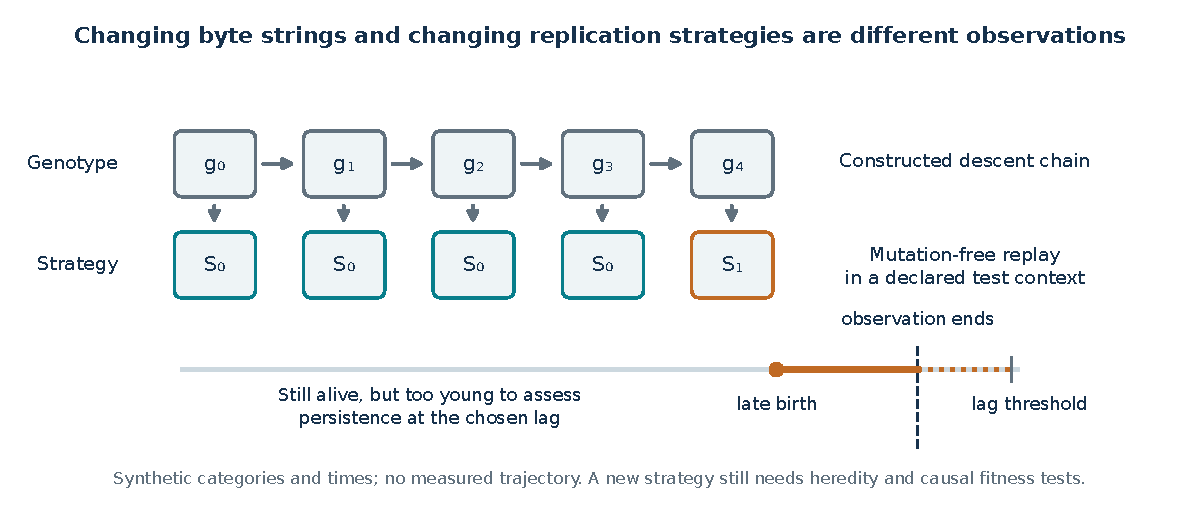
\includegraphics[width=\textwidth]{figures/measurement-limits.pdf}
\caption{Original categorical illustrations of two measurement limits.
Distinct genotypes can be equivalent under a declared mutation-free test
panel; a newly distinguished strategy still needs heredity and causal
reproductive-effect tests. This distinction is motivated by
\citet{Standish2003,Taylor2016}. The separate lower timeline shows a lineage
alive at observation cutoff but younger than the persistence lag; its status
at that lag is unresolved. The dotted future segment is unobserved, not
continued survival. Categories and times are constructed, not measured data.}
\label{fig:measurement}
\end{figure}
Figure~\ref{fig:measurement} separates observable genotype change, operational
strategy change, and incomplete follow-up.

\subsection{From description to causal evidence}
An analysis label should follow a controlled comparison. One useful design
compares A alone, B alone, and A+B under specified placement, duration,
permissions, and resource conditions. Further substitutions can disable an
instruction source, replace copied data, or alter whether a neighbor responds.
The goal is to locate the causal dependency, not to preserve a preferred
ecological classification.

Such tests also reveal the limits of static genome analysis. The same bytes
can support different outcomes in different contexts, while distinct genomes
can implement similar reproductive behavior. Functional equivalence must
therefore be defined relative to a test panel and reported at that resolution.
An empirical claim of innovation should identify the newly expressed behavior,
its heredity, its persistence, and its reproductive consequences. No finite
run establishes indefinite innovation, and a bounded fixed-state system has
only finitely many distinct states. Scale extension and sensitivity analysis
strengthen a finite claim without turning it into a proof of unboundedness.

\FloatBarrier
\section{Emergent boundaries, conserved flows, and operational individuality}
\label{sec:boundaries}
The second literature pass asks what previous systems required to construct
and maintain boundaries, account for resources, organize groups, and detect
individuality. Its fifteen-work corpus is bounded design input, not a novelty
assessment. Detailed source versions, inspected sections, failed retrievals,
and screened leads accompany the three repository reports. A membrane, a
write permission, a cooperating group, and an observer's candidate individual
are distinct objects. Finding one does not establish the others.

\begin{figure}[!htbp]
\centering
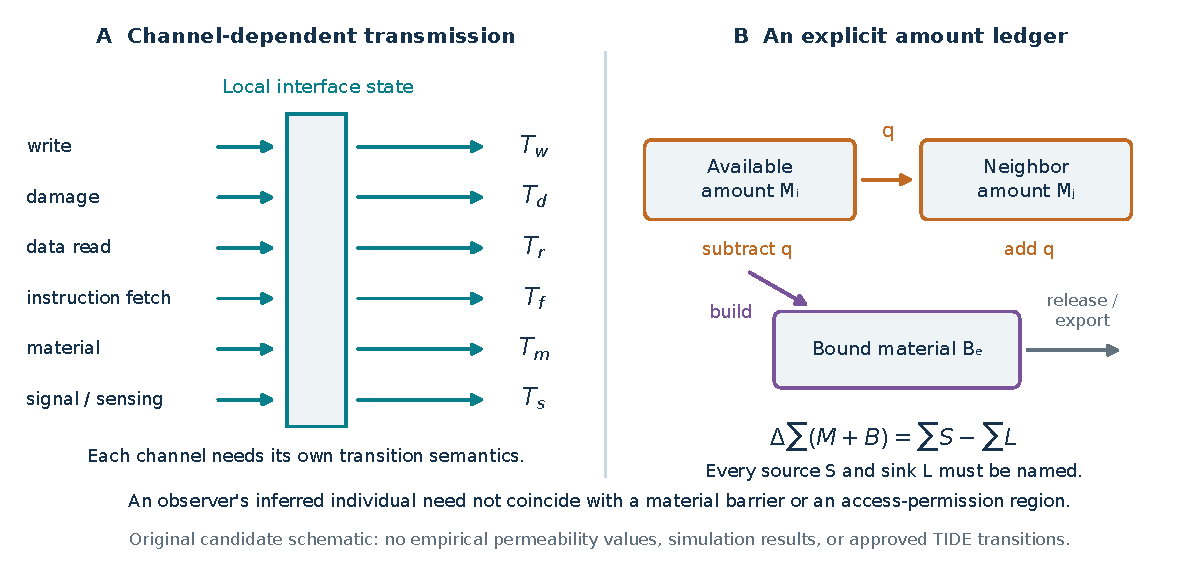
\includegraphics[width=\textwidth]{figures/graded-boundaries.pdf}
\caption{Original design vocabulary for channel-dependent boundaries and
explicit accounting. The $T_c$ symbols denote separate transmission rules,
not measured values or a required probability representation. For a declared
material, internal transfers debit and credit the same quantity; construction
can move it into bound material, while release returns it to a tracked pool
or an explicit sink. The equation is an accounting identity for this proposed
representation, not a model reproduced from the literature. Neither the
interface variable nor these transitions are an approved TIDE contract.}
\label{fig:graded-boundaries}
\end{figure}

\subsection{What emerges, and what the chemistry already supplies}
Varela, Maturana, and Uribe's model constructs a membrane-like enclosure from
local production, movement, bonding, and disintegration
\citep{Varela1974}. The constitutive chemistry already distinguishes substrate,
catalyst, and link components. Its example concerns self-maintaining enclosure;
it is not a demonstration that cellular reproduction or arbitrary selective
permeability emerges from unconstrained matter. Maintenance also depends on
what may cross the constructed chain. Species-selective transport is supplied
by the model even when the enclosure itself is assembled dynamically.

The replication study by \citet{McMullinVarela1997} exposes a consequential
missing rule: chain-based bond inhibition was not specified in the earlier
description, but recovering it from historical code was critical to the
reported behavior. Its application must distinguish free links from singly
bonded links; blocking the latter interferes with repair. This is a concrete
warning against treating a short list of attractive ingredients as a complete
transition system. Which partner is eligible, which neighboring bonds inhibit
an event, and which failed events leave state unchanged can determine whether
a boundary forms and survives.

Ono and Ikegami's 2000 model offers a different construction
\citep{OnoIkegami2000}. It is a one-dimensional stochastic lattice with many
particles per site, not the separate two-dimensional 1999 model sometimes
associated with the same authors. Metabolism produces membrane material;
local membrane accumulation affects escape, and fixed differences in species
mobility change the mode of reproduction. The work reports outward production
of new cells and internal division under different mobility conditions.
Integer particle exchange in its movement algorithm is relevant to accounting,
but the ordering and event probabilities remain stochastic. Dynamic membrane
thickness and graded leakage do not by themselves establish evolution of the
transport law: relevant coefficients are specified by the investigator.

Hutton's 2007 artificial chemistry demonstrates evolvable self-reproducing
cells with a supplied loop membrane and genetic construction machinery
\citep{Hutton2007}. The initial replication system and its reaction rules are
designed; the chosen loop membrane does not supply the self-assembly and repair
of the autopoietic example. Molecular size helps distinguish what passes the
membrane from what is retained. This provides a useful contrast: inheritance
and modification of a replication procedure can be studied even when the
initial boundary and the allowed transport categories are given. It should
not be described as spontaneous origin of either the entire cell or an
unrestricted permeability mechanism.

Together these models support separating at least three questions. Does a
boundary assemble and persist under component turnover? Does its structure
alter transport continuously or categorically? Can the relation between
structure and transport itself vary heritably? A designed interaction can
answer the first question without answering the third. Conversely, making
every cross-boundary operation costly need not create a viable boundary:
construction, repair, nutrient access, and waste release must remain compatible.

\subsection{Perception, local dependence, and propagation}
Egbert, Barandiaran, and Di Paolo model chemotactic behavior coupled to
metabolic state \citep{Egbert2010}. Their compartment, transport coupling, and
movement control are provided by the model. The result concerns how behavior
can depend on viability-related dynamics; it does not show an emergent membrane
or a universal protection-versus-perception tradeoff. Local uptake of a field
value also does not specify how the field arrived at that location. A sensing
rule and a signal propagation rule are separate commitments.

Flow-Lenia directly evaluates a convolution-defined neighborhood and uses
local affinity gradients to transport activation mass
\citep{Plantec2025}. The finite spatial support of a local rule limits its
one-step dependencies. It does not imply that information travels by the same
mechanism as material, that an intervening barrier occludes the sensed field,
or that the mathematical continuous-time limit has a finite signal speed.
Such conclusions require explicit update timing and field dynamics. The
mass-transport mechanism supports persistent spatial patterns, but a contour
of activation is not automatically a membrane whose permeability or sensing
cost is maintained by those patterns.

For TIDE, write access, damage, data reading, instruction fetch, material
exchange, and signal access therefore need individual semantics
(Figure~\ref{fig:graded-boundaries}). A candidate design could couple some
channels to locally produced boundary material. It must still say whether
transmission is a rate, a capacity, a deterministic coefficient, a stochastic
event probability, or a permission predicate. The literature does not supply
one interchangeable numerical parameter for all these channels, nor does this
pass establish a general tradeoff curve between protection and perception.

\subsection{Conservation and limited resources are different constraints}
Coreworld's local execution credit, Avida's resource-mediated computational
opportunities, Stringmol's two historical resource formulations, and
Flow-Lenia's activation mass constrain activity in different ways
\citep{Rasmussen1991,OfriaWilke2004,StringmolSpec2010,Hickinbotham2021,Plantec2025}.
A capped or replenished credit is not automatically conserved material.
Calling every scalar ``energy'' can conceal its source, clock, ownership,
transport rule, and eventual destination.

The Coreworld chapter replenishes local execution resources from outside and
removes execution pointers when resources fail. It distinguishes snapshot
and sequential memory effects; the exact distribution of a neighborhood
debit is not fully specified in the chapter. Avida explicitly supplies resource
and environmental machinery that can change computational rewards. Neither
example establishes that every copied instruction consumes a conserved local
building block, or that removing a resource constraint leaves all other
selection pressures unchanged.

The 2010 Stringmol specification uses a global energy mechanism and an
abundant supply of free symbols \citep{StringmolSpec2010}. The 2021 spatial
experiment instead schedules one opcode per bound pair per timestep and does
not retain that energy gate \citep{Hickinbotham2021}. Copying and cleavage in
these models should not be reinterpreted as conservation of total string
length or molecule number. In the 2021 spatial model, stochastic decay and
vacancy-dependent placement provide turnover and spatial limitation, but they
are different from a closed
material budget. The published extinctions also preclude treating this
combination as a guarantee of persistence.

For a proposed integer material ledger, a transfer of $q$ from $i$ to $j$
would pair $m_i'=m_i-q$ with $m_j'=m_j+q$, subject to available amount and
destination capacity. Multiple simultaneous requests require an allocation
rule before either side is committed. Conservation additionally needs explicit
sources, sinks, material bound into structures, and release on destruction.
These equations are design proposals, not claims that the cited systems use
the same representation. Rounding, overflow, rejected transfers, and
same-step availability must be settled before claiming exact synchronous
accounting. A floating-point conservation argument alone does not establish
bit-for-bit conservation in an integer implementation.

\subsection{Groups that develop inside supplied grouping machinery}
DISHTINY is particularly informative for candidate option B because cells are
given while their behaviors and spatial cooperation can evolve
\citep{MorenoOfria2022}. The inspected 2022 system nevertheless supplies
hereditary group identifiers, nested grouping levels, group aging, and
resource-reward mechanisms, as well as four directional controllers per cell.
Cooperation and reproductive organization can
emerge within that environment without demonstrating that group membership
itself was inferred from unlabeled material interactions. Its controls with
even resource inflow also allow cooperation, with hereditary recognition,
imposed aging, and local competition retained. The tested reward wave is
therefore not required for every observed cooperative behavior under those
remaining conditions.

The paper-linked implementation adds further semantics: floating-point
resource values, staged contributions, and randomized order within cells or
when resolving conflicts. A code default for resource decay differs from the
article's numerical description. These are documented code observations,
not substituted facts about every published run. An integer translation
requires a separate transition contract and validation of timing, rounding,
priorities, and accounting; specifying these conventions alone does not
establish ecological equivalence.

A group transition contract should state what a joining or departing member
transfers: control, resources, territory, identifiers, or only observable
links. Fission must decide how claims and stored quantities are partitioned;
death must specify which structures and claims survive. Failed joins,
conflicting claims, and simultaneous fissions require effects as explicit as
successful reproduction. The selected sources do not provide a generic
join/leave/divide API that can be adopted without these decisions. Under
option B, per-site ownership would remain a supplied primitive; emergence of
body shape and cooperation would be the phenomenon to test.

\subsection{Measuring individuality without physical role labels}
Information-theoretic individuality evaluates dependence between a candidate
system, its environment, and their temporal states \citep{Krakauer2020}.
Continuous scores and nested candidate systems can express degrees of
individuality. They still require the observer to specify variables, a
candidate partition, temporal resolution, and probability estimates. The
authors note that relevant autonomy scores can grow with system size; a
precise boundary then requires an additional size cost or regularizer. A
continuous score is not an algorithm that automatically discovers a unique
spatial body or assigns independently varying permeability to its channels.

Fontana and Buss study constructive organizations of interacting expressions
\citep{FontanaBuss1993}. The inspected source is their 1993 working-paper
precursor of the 1994 article. Closure and self-maintaining organization concern
relations among the chosen objects and reactions, not necessarily a spatial
enclosure. Chemical organization theory formalizes closure together with
feasible sustaining production flux \citep{Dittrich2005}. Here the detailed
definitions are taken from the explicitly labeled 2005 preprint; the longer
2007 journal typesetting was not retrieved. Species-set closure is categorical
even when its flux constraints involve continuous values. Neither framework
identifies geometric membrane permeability from an arbitrary image or a
short observed event graph.

BFF's replicator detector supplies a useful contrasting operational test
\citep{Knierim2026}. It evaluates a declared finite family of copying
trajectories and agreements between produced tapes. Its input tape units,
replay protocol, and thresholds are supplied. Consequently it detects a
particular replication property, not general individuality. The inspected
paper's branch-count description is internally inconsistent, and a current
official-code branch differs from the preprint thresholds. Neither code
inspection nor a detector label is a substitute for reproducing the stated
version of the test.

Computational costs depend on the observer. For a fixed candidate partition,
information measures require trajectory counts or density estimates; searching
all subsets of $n$ components can expose $2^n$ candidates before estimation.
This is a combinatorial design estimate, not a benchmark reported by the
papers. Closure tests require a specified reaction universe; feasible
self-maintenance adds flux constraints, while enumerating organizations can
again be combinatorial. Unobserved reactions cannot be certified impossible
merely because replay logs contain no examples. A reproducible detector needs
the relevant initial state and transition rules, not just a record that a
birth was announced.

Thus ``label-free'' should mean that ecological or individual labels do not
drive the physical transitions. Observation still has choices. Replayable
logs should permit candidate regions, event provenance, amounts, lags, and
coarse-graining to be varied afterward. Any soft membership weights or
cross-boundary flux summaries proposed for TIDE remain analysis candidates;
they should not silently become ownership grants, fitness rewards, or
requirements that evolution produce a preferred kind of individual.

\FloatBarrier
\section{Research synthesis and implications for TIDE}
\subsection{Common questions across substrates}
The three substrate classes expose different parts of the same constructive
problem. Soft systems make causality and heredity inspectable; hardware makes
contact, manufacturing, and control errors unavoidable; wet systems expose
whether maintenance, compartmentalization, and information copying can operate
together chemically. No single demonstration should substitute for the
integration problem addressed by another class.

Across them, five questions remain useful. First, what is the reproducing
unit, and can that unit change? Second, which resources and environmental
services are supplied? Third, how does inherited organization affect future
opportunities? Fourth, which processes are controlled by an external optimizer
or experimenter? Finally, which observation would falsify the proposed
mechanism? These questions organize comparisons without requiring all systems
to use the same substrate or pursue the same objective.

For soft artificial life, a productive priority is to make mechanistic claims
sharper rather than to add more life-like vocabulary. New instructions,
environmental gradients, ecological rewards, or learned evaluators enlarge
the design space, but also add assumptions. Their value is established by
controlled contrasts that explain what becomes possible and what changes in
measured outcomes. Negative results can identify a missing expressive
capability, an unfavorable ecological regime, or a limitation in the observer.

\subsection{TIDE's present position}
TIDE currently has research documentation and an earlier local prototype;
the fresh C++ kernel has not been implemented. The project has selected an
individual-CPU local address-based VM, pointer-directed byte copying,
allocation that occupies public lattice space before division, and a two-phase
synchronous default. It begins with a supplied ancestor. Ecological labels
must not determine physical behavior. These are project decisions, not results
proved by the reviewed literature.

The instruction-level contract remains open. In particular, read visibility,
conflict resolution, newborn scheduling, reclamation, and mutation require
explicit transitions including failure effects. Working defaults such as
readable residual bytes and CPU-only costs remain experimental variables.
Choosing a reference CPU implementation and deterministic replay helps
separate implementation discrepancies from intended changes in the model.

\subsection{Candidate directions and discriminating tests}
The current design discussion asks whether channel-dependent boundaries can
be constructed and maintained by local dynamics. Candidate ``option B'' keeps
execution threads and per-site ownership as supplied primitives, while leaving
body extent, shape, territorial division, and multi-thread grouping open to
evolution. It therefore leaves some units given while seeking emergence at
other scales. It is a discussion direction, not an amendment to the agreed
kernel contract. The second literature pass supplies design constraints and
failure cases without assessing novelty.

One useful controlled comparison from the earlier pass remains:
\begin{quote}
Starting from a supplied ancestor, how do local data-reading and
instruction-fetch permissions affect the appearance and persistence of
functionally distinct replication strategies?
\end{quote}
This is a proposed research question. Self-only, neighbor-data access, and neighbor-data-plus-fetch
conditions could be compared while holding write permissions and other rules
fixed. The ancestor must be viable across the relevant comparison. Mutation-free
examples establish expressive capacity before evolutionary runs begin.

Extending that comparison to constructed boundaries requires additional
decisions: what changes each channel's transmission, which material or work
is consumed, how decay and repair affect access, and how simultaneous requests
are resolved. Group formation then needs separate join, leave, fission,
death, and transfer semantics. An observer's inferred individuality should
remain an analysis result rather than an input granting physical privileges.

Two subordinate questions are worth retaining. Does readable residual code
support heritable replication opportunities after its producer dies, or merely
alter occupation and transient copying? Are observed dependencies robust to
the specified sequential-update comparison and alternative conflict policies?
The first requires causal removal/replacement of recorded bytes; the second
requires matched execution budgets and distributional comparisons across
seeds. Neither has been answered by TIDE experiments.

The minimum evidence package should identify all seeds and configurations,
archive the kernel revision, retain lifecycle and material-provenance records,
and report stagnation and extinction alongside surviving trajectories.
Implementation acceptance concerns semantics, locality, accounting, and
replay. Research acceptance must also allow a well-supported negative answer;
observing a desired ecological role should not be an engineered requirement.

\section{Conclusion}
Artificial life contains a family of constructive experiments rather than a
single route from simple rules to complete life. Self-organization,
self-reproduction, heredity, adaptation, and continuing innovation remain
distinct achievements. Digital programs and automata are especially useful
for tracing how inherited organization changes its own reproductive pathways;
robotic and biochemical work clarifies which constraints disappear when that
organization is simulated. The immediate opportunity for TIDE is a precise,
replayable investigation of replication access and ecological feedback, with
measurements that distinguish changing bytes from changing strategies. The
literature supports this as a tractable research direction while leaving its
outcome open.

\FloatBarrier
\clearpage
\appendix
\section{An archived shared-memory probe in historical context}
\label{sec:probe}
This appendix reanalyzes an existing exploratory prototype, separate from the
fresh TIDE kernel and the literature evidence above. No simulations were
rerun for the review. The local record contains 140 output files: 20 baseline,
100 intervention, and 20 ownership-comparison files. Ten ownership-comparison
cases repeat an earlier condition, leaving 130 distinct seed/configuration
tuples. The source and raw outputs remain local; the review bundle includes
the ten plotted records, their source filenames and SHA-256 hashes, and the
extraction and plotting scripts.

\subsection{What the recorded comparison establishes}
The probe uses a $48\times48$ torus, 32 bytes per site, separate execution
pointers, and a supplied 17-byte ancestor. Updates run sequentially in CPU
birth order, four instructions per CPU per round; this is not TIDE's chosen
two-phase default. Figure~\ref{fig:probe} compares unrestricted and claimed
writes under one shared setting: local removal above one CPU per site,
maximum age 200 rounds, successful-write coverage before spawn, and per-byte
copy mutation 0.003. All five seeds per condition are shown.

\begin{figure}[!htbp]
\centering
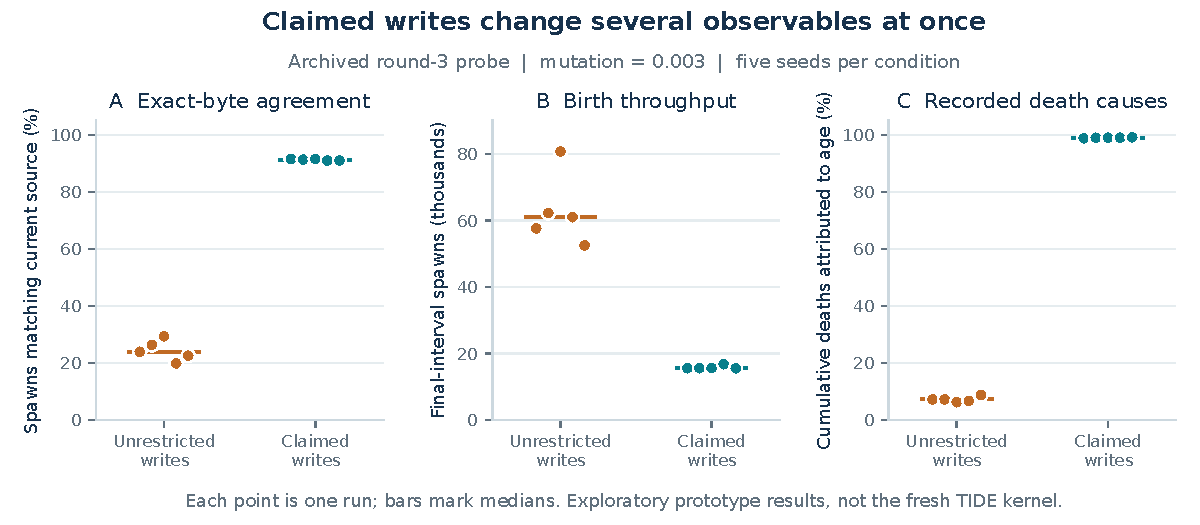
\includegraphics[width=\textwidth]{figures/probe-tradeoffs.pdf}
\caption{Reanalysis of archived round-3 prototype outputs, not a literature
figure or fresh TIDE result. Each point is one seed; horizontal bars are
medians, not confidence intervals. A compares target bytes with the executing
CPU's current memory site at spawn; it does not measure functional heredity.
A and B use the last 2,000-round interval of 20,000-round runs; C uses
cumulative death counters. Claimed writes jointly change body protection,
allocation ownership, vacancy access, and transfer rules, so this is a bundled
intervention. Values are read from the original logs; byte percentages retain
their original two-decimal rounding.}
\label{fig:probe}
\end{figure}

Under mutation, claimed writes raise final byte agreement from approximately
20--29\% to 91--92\%, while reducing final birth throughput by 3.38--5.17 times
for the same seed identifiers. The random-event histories need not remain
coupled across these treatments. Almost all recorded deaths under claimed
writes are attributed to age; most under unrestricted writes are local-cap
removals after arrivals by birth or movement. Overwriting bytes itself does
not remove a CPU in this implementation. The plot therefore supports a change
in several recorded observables, not a demonstrated gain in evolutionary
capacity or the isolated effect of body protection.

\subsection{How earlier systems addressed the same questions}
\textbf{Construction before new execution.}
Tierra's later V5.0 manual explicitly motivates a movement-count threshold
before division by the production of empty offspring when it is absent
\citep{RayManual1998}. Repeated writes to one address can satisfy its documented
count; this differs from the probe's distinct-offset coverage. The manual's
two descriptions disagree about the size denominator, so the exact threshold
requires version-specific code inspection. Avida separately checks allocation,
size, executed-parent fraction, and copied-offspring fraction before division
\citep{OfriaWilke2004}. Its main text and appendix also give different fractions.
The transferable distinction is between reservation, construction evidence,
and reproductive viability, not a universal numerical gate.

\textbf{Population survival after reproduction fails.}
Avida's authors explicitly warn that birth-only replacement can leave a
population present after self-replication is lost, and describe optional
death after a number of executed instructions \citep{OfriaWilke2004}.
Coreworld/Venus instead limits execution through local renewable resources;
resource failure and certain instructions remove pointers, while other rules
inject them \citep{Rasmussen1991}. Spatial Stringmol has stochastic decay and
vacancy-dependent product placement, yet still reports extinctions
\citep{Hickinbotham2021}. These are different turnover processes. An independent
death clock can reveal reproductive failure rather than rescue the population.

\textbf{Overwrite and interaction.}
Coreworld's authors report seeded replicators losing their reproductive
organization through noise and mutual overwriting \citep{Rasmussen1991}.
Tierra protects body and daughter-memory writes while permitting foreign
execution \citep{Ray1991}. This is a historical architectural contrast, not a
controlled demonstration that ownership is necessary. For functional diagnosis,
Avida tests descendant viability and Stringmol replays mutation-free reactions
in both orientations \citep{OfriaWilke2004,Hickinbotham2021}. The latter procedure
is particularly useful when solitary viability would miss partner dependence.

\subsection{Corrections and discriminating next controls}
The source audit narrows several initial interpretations. Baseline freezes
occur with 1,024 CPUs on 2,304 sites, so full occupancy is not necessary.
Successful-write coverage records historical writes, not the final integrity
or provenance of the destination. A count of surviving CPUs that previously
spawned is not the interval birth count. Memory-string richness includes
relics and allocations. Finally, the stored digest omits RNG state, ages,
coverage masks, and other future-relevant fields; matching recorded digests
does not establish full-state deterministic replay.

The next controls should separate three questions: whether division requires
reservation, counted writing, or distinct-address coverage; whether turnover
continues when births are suppressed; and whether body protection or
single-writer allocation causes the observed throughput change. Mutation-free
descendant and partner replay should accompany byte metrics. These are
proposed experiments, not changes to the agreed kernel contract. The detailed
source comparison and audit remain in the repository's research notes.

\FloatBarrier
\clearpage
\begingroup
\small\raggedright
\bibliographystyle{plainnat}
\bibliography{references}
\endgroup
\end{document}
